% Copyright 2004 by Till Tantau <tantau@users.sourceforge.net>.
%
% In principle, this file can be redistributed and/or modified under
% the terms of the GNU Public License, version 2.
%
% However, this file is supposed to be a template to be modified
% for your own needs. For this reason, if you use this file as a
% template and not specifically distribute it as part of a another
% package/program, I grant the extra permission to freely copy and
% modify this file as you see fit and even to delete this copyright
% notice. 

\documentclass{beamer}

% There are many different themes available for Beamer. A comprehensive
% list with examples is given here:
% http://deic.uab.es/~iblanes/beamer_gallery/index_by_theme.html
% You can uncomment the themes below if you would like to use a different
% one:
%\usetheme{AnnArbor}
%\usetheme{Antibes}
%\usetheme{Bergen}
%\usetheme{Berkeley}
%\usetheme{Berlin}
%\usetheme{Boadilla}
%\usetheme{boxes}
%\usetheme{CambridgeUS}
%\usetheme{Copenhagen}
%\usetheme{Darmstadt}
%\usetheme{default}
%\usetheme{Frankfurt}
%\usetheme{Goettingen}
%\usetheme{Hannover}
%\usetheme{Ilmenau}
%\usetheme{JuanLesPins}
%\usetheme{Luebeck}
\usetheme{Madrid}
\usepackage[utf8]{inputenc}
\usepackage[T1]{fontenc}
\usepackage[english]{babel}
%\usetheme{Malmoe}
%\usetheme{Marburg}
%\usetheme{Montpellier}
%\usetheme{PaloAlto}
%\usetheme{Pittsburgh}
%\usetheme{Rochester}
%\usetheme{Singapore}
%\usetheme{Szeged}
%\usetheme{Warsaw}
\usepackage{subcaption}
\usepackage{caption}
\usepackage{graphicx}

\title{Fast reinforcement learning for energy-efficient wireless communications}

% A subtitle is optional and this may be deleted
\subtitle{INF8225 – Project}

\author{Farnoush~Farhadi \and Juliette~Tibayrenc}
% - Give the names in the same order as the appear in the paper.
% - Use the \inst{?} command only if the authors have different
%   affiliation.

\institute[Polytechnique Montreal] % (optional, but mostly needed)
{Polytechnique Montreal}
% - Use the \inst command only if there are several affiliations.
% - Keep it simple, no one is interested in your street address.

\date{April 2016}
% - Either use conference name or its abbreviation.
% - Not really informative to the audience, more for people (including
%   yourself) who are reading the slides online

\subject{Project}
% This is only inserted into the PDF information catalog. Can be left
% out. 

% If you have a file called "university-logo-filename.xxx", where xxx
% is a graphic format that can be processed by latex or pdflatex,
% resp., then you can add a logo as follows:

% \pgfdeclareimage[height=0.5cm]{university-logo}{university-logo-filename}
% \logo{\pgfuseimage{university-logo}}

% Delete this, if you do not want the table of contents to pop up at
% the beginning of each subsection:


\AtBeginSubsection[]
{\begin{frame}<beamer>{Contents}
    \tableofcontents[currentsection,currentsubsection]
  \end{frame}}

% Let's get started
\begin{document}

\begin{frame}
  \titlepage
\end{frame}

\begin{frame}{Motivation}
\begin{itemize}
\item Practical application of Markov Decision Processes (MDPs)
\item Explore algorithm variants and compare results
\end{itemize}
\end{frame}

\begin{frame}{Contents}
  \tableofcontents
  % You might wish to add the option [pausesections]
\end{frame}

% Section and subsections will appear in the presentation overview
% and table of contents.
\section{The article} 
\subsection{Context}
\begin{frame}{Context}
\begin{itemize}
\item several ways to optimize power consumption while transmitting delay-sensitive information
\begin{itemize}
\item on the software side$\dots$
\item and on the hardware side
\end{itemize}
\item but no strategy to ally both
\item Unknown dynamic environments
\begin{itemize}
\item Dynamic traffic and channel conditions
\item Lack of statistical knowledge of dynamics
\item Fast learning algorithms
\end{itemize}
\item Heterogeneous multimedia data
\begin{itemize}
\item Different deadlines, priorities, dependencies
\end{itemize}
\end{itemize}
\end{frame}

\subsection{Problem}
\begin{frame}{Problem}
Find a way to solve the optimization problem
(balancing the constraints of low power consumption and low transmission time)
\begin{figure}
\begin{center}
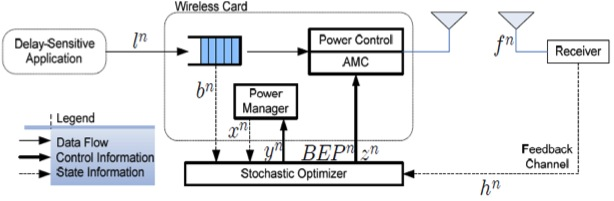
\includegraphics[width=12cm]{problem_schema.jpg}
\caption{Power consumption minimization s.t buffer delay constraint (from the original article)}
\end{center}
\end{figure}
Rule: Average buffer delay is proportional to average buffer occupancy
\end{frame}

\subsection{Proposed solution}
\begin{frame}{Proposed solution}
\begin{itemize}
\item Power management problem $\equiv$ MDP
\item Separate known and unknown components (generalize* the PDS concept)
\item Use reinforcement learning to solve the DPM problem
\end{itemize}
\end{frame}

\section{Some theory}
\subsection{Related algorithms}
\begin{frame}{Related algorithms}
\begin{itemize}
\item Value iteration and policy iteration
\begin{itemize}
\item iterative algorithms
\item aim: find the optimal policy (directly or indirectly by optimizing the value function)
\end{itemize}
\item Reinforcement learning \& Q-learning
\begin{itemize}
\item dynamics \& reward function initially unknown
\item Q-learning: learn the best policy from history
\end{itemize}
\end{itemize}
\end{frame}

\section{A few results}
\begin{frame}{A few results}
\begin{figure}
\begin{center}
\begin{subfigure}{.5\textwidth}
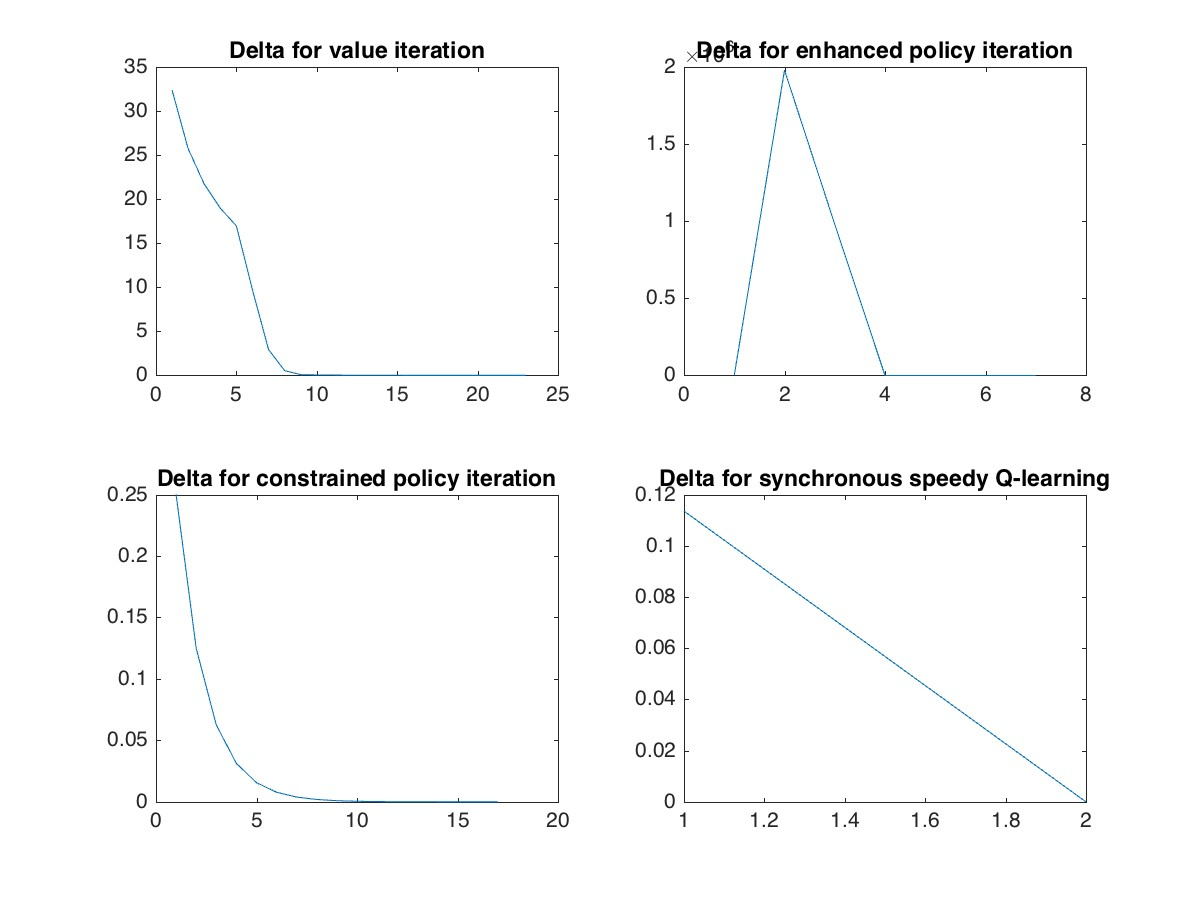
\includegraphics[width=1\linewidth]{deltas.jpg}
\end{subfigure}%
\begin{subfigure}{.5\textwidth}
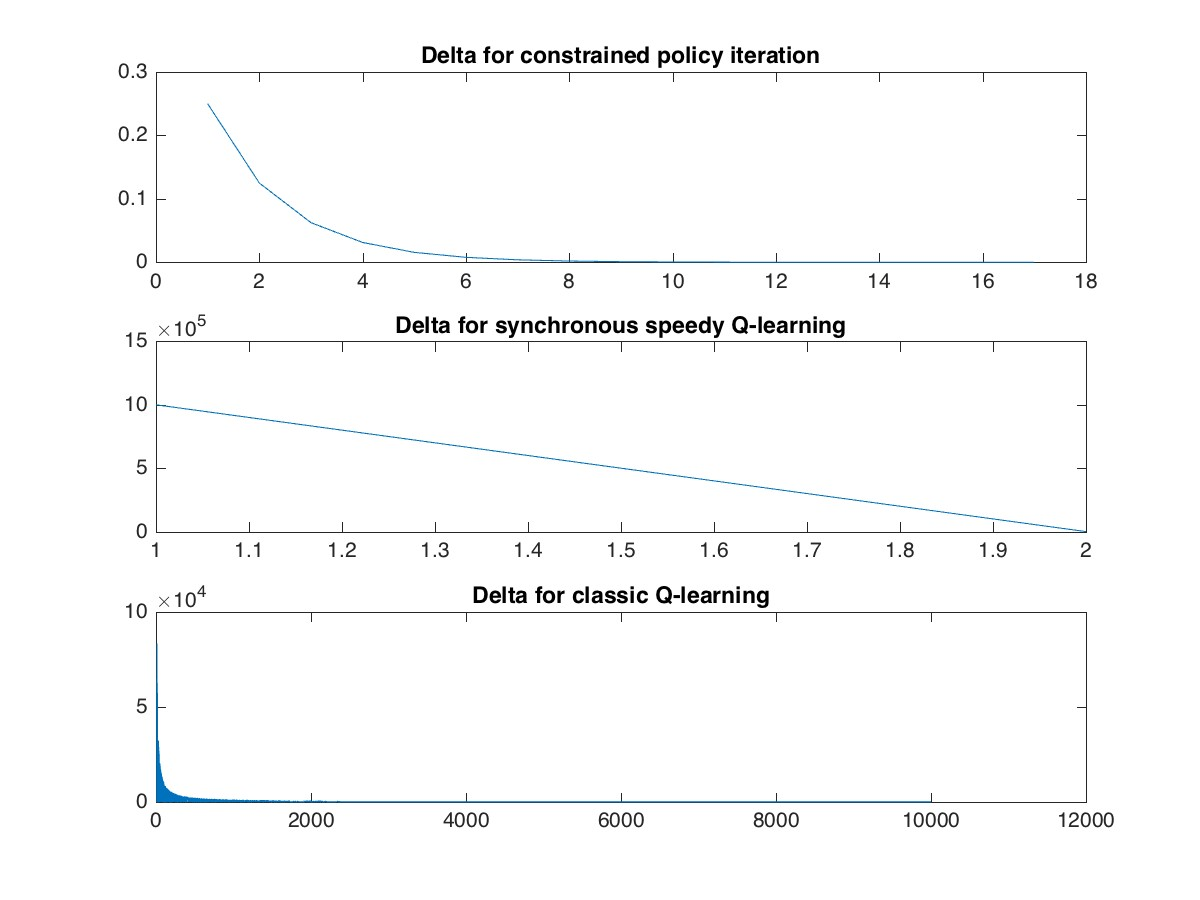
\includegraphics[width=1\linewidth]{deltas_the_sequel.jpg}
\end{subfigure}
\caption{Comparing the required number of iterations to get to the optimal policy}
\end{center}
\end{figure}
Caution: not the measure that's the most indicative of performance
\end{frame}

\subsection{Subproblem: obtaining the reward matrix}
\begin{frame}{Reward matrix}
\begin{itemize}
\item Reward obtained for getting to one state?
\item $\implies$ algorithm to compute the reward matrix
\end{itemize}
\end{frame}

\begin{frame}
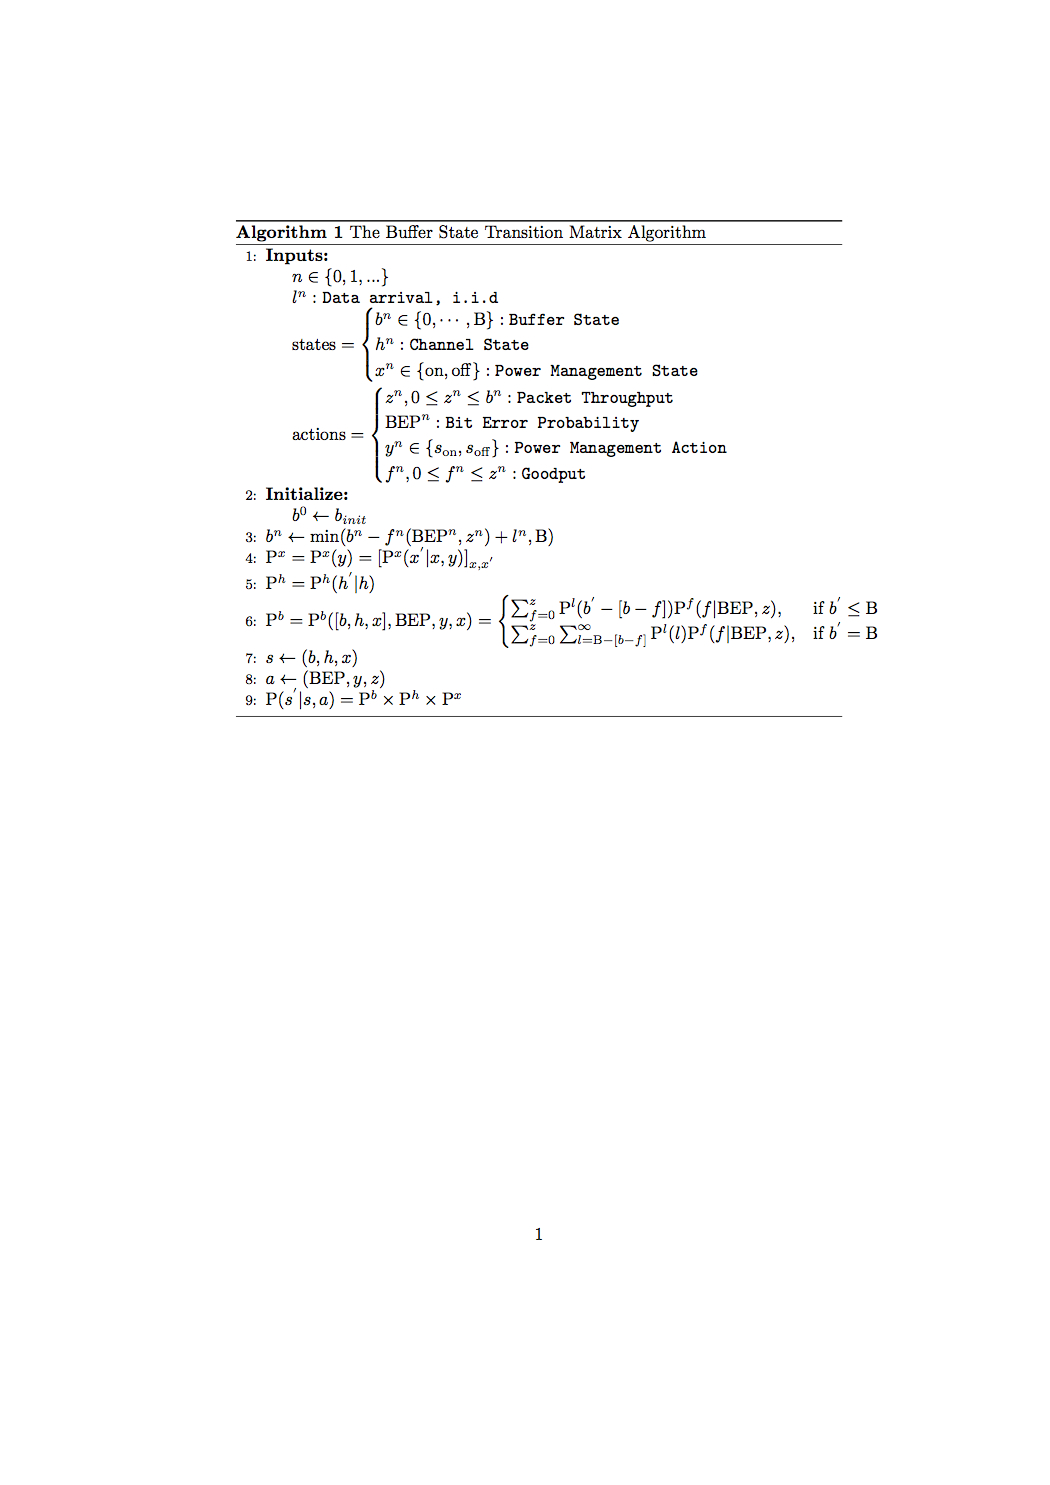
\includegraphics[trim={2cm 10cm 0 2cm},width=12cm]{pseudocodes.jpg}
\end{frame}

\section{Conclusion}
\begin{frame}{Conclusion}
The authors:
\begin{itemize}
\item Considered the problem of energy-efficient point-to-point transmission of delay sensitive over a fading channel. 
\item Proposed a unified reinforcement learning solution for finding the jointly optimal power-control, AMC, and DPM policies when the traffic arrival and channel statistics are unknown. 
\item Exploited the structure of the problem:
\begin{itemize}
\item introducing a post-decision state
\item eliminating action-exploration
\item enabling virtual experience to improve performance
\end{itemize}
\end{itemize}
\end{frame}

\begin{frame}{Conclusion}
We:
\begin{itemize}
\item synthetised this work \& reproduced results
\item focused on the reward matrix subproblem
\item implemented other approaches to solve the problem
\end{itemize}
Proposed algorithm outperforms existing solutions;
our first algorithm outperforms it on some measures but don't present the same advantages.
\end{frame}

\section{Possibilities for a future work}
\begin{frame}{Possibilities for a future work}
Can be applied to any network or system resource management problem involving controlled buffers.
$\implies$ Apply it in a system with multiple users by integrating the single-user optimization with one of the multi-user resource allocation framework (ex: uplink or downlink transmission in cellular systems)
\end{frame}

\section{References}
\begin{frame}{References}
\begin{enumerate}
\item Mastronarde, N. and Van der Schaar, M., 2011. Fast reinforcement learning for energy-efficient wireless communication. Signal Processing, IEEE Transactions on, 59(12), pp.6262-6266.
\item Wiering, M. and Schmidhuber, J., 1998. Fast online Q (λ). Machine Learning, 33(1), pp.105-115.
\item Ghavamzadeh, M., Kappen, H.J., Azar, M.G. and Munos, R., 2011. Speedy Q-learning. In Advances in neural information processing systems (pp. 2411-2419).
\end{enumerate}
\end{frame}

\end{document}
